\section{实验装置设计}
本章节主要介绍单摆实验装置的设计,包括单摆实验装置的设计、AI辅助系统的设计以及实验装置的系统误差分析。
\subsection{单摆实验装置设计}

本实验采用精密单摆装置,其主要构成包括:线长调节轮盘、高精度摆线、金属支撑杆、稳固底座、精密刻度盘及标准带孔摆球。装置设计遵循物理实验精确性和操作便捷性原则。

线长调节轮盘内部集成长度约1米的高强度细线,通过精密啮合机构实现摆线长度的连续可调与精确控制。根据单摆理论,摆线的有效长度被定义为线段长度与悬挂钢球半径之和,这一参数对实验测量结果具有决定性影响。

支撑系统由直径7.5 mm的高强度金属杆构成,提供足够的刚性支撑,有效减小实验过程中的系统振动误差。底座及刻度盘采用一体化加厚设计,显著提升整体结构稳定性,同时刻度盘上精确标记的角度刻度使摆动初始角度的设定和读数更为精确,满足定量实验需求。

实验用摆球包含多种材质和规格,具体包括:带孔钢球(直径约19 mm,质量约27 g,1颗)、带孔钢球(直径约13 mm,质量约6.5 g,2颗)、带孔塑料球(直径约27 mm,质量约9 g,1颗)、带孔塑料球(直径约19 mm,质量约4 g,1颗)。所有摆球均为中心穿孔设计,便于摆线安装与固定,确保摆动过程中质量分布的均匀性。

该装置整体高度为41 cm,底座尺寸为11.5 cm×9 cm,净重约570 g。整体结构紧凑、参数稳定、操作简便,适用于教学实验及科研工作中重力加速度测量、简谐运动分析等相关物理实验。
\begin{figure}[H]
    \centering
    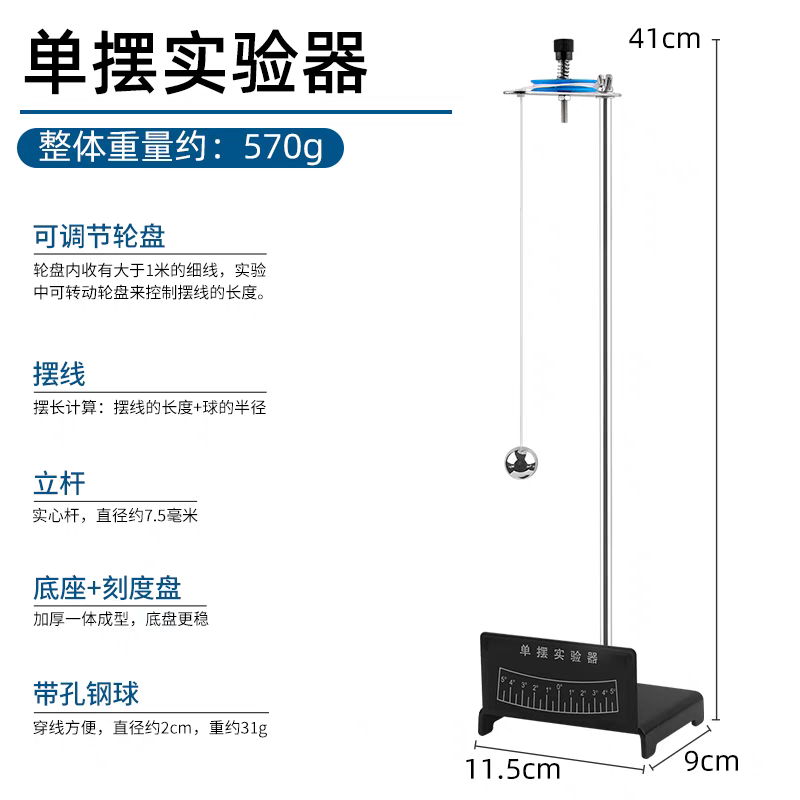
\includegraphics[width=0.45\textwidth]{figures/单摆实验装置1.jpg}
    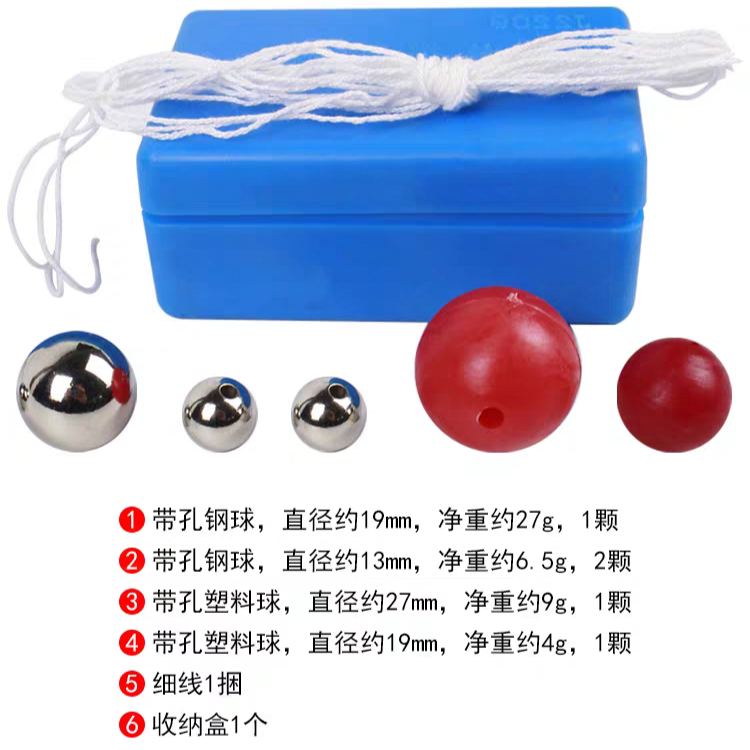
\includegraphics[width=0.45\textwidth]{figures/单摆实验装置2.jpg}
    \caption{单摆实验装置}
    \label{fig:pendulum_device}
\end{figure}

\subsection{AI辅助系统设计}

针对上文的单摆实验装置,本项目设计了基于深度学习的单摆实验AI辅助系统,旨在通过计算机视觉技术实现单摆运动的\textbf{自动跟踪、数据采集与分析,提高物理实验的精确性}。该系统采用YOLO目标检测算法精确识别并追踪摆球位置,通过多种数据分析方法计算单摆周期与重力加速度,实现了从视频输入到物理参数计算的完整自动化流程。系统的实现包含数据集采集与处理、模型训练与评估以及软件实现三大部分,整套系统将AI技术与物理实验有机结合,有效解决了传统人工观测耗时费力且精度有限的问题。

\subsubsection{数据集的采集与处理}

为确保模型的鲁棒性,本团队在多种环境条件下采集装置的训练数据集。数据集由100张高质量图像组成,按照4:1的比例划分为训练集(80张)和验证集(20张),以确保模型具有良好的泛化能力,数据标注采用labelImg工具进行人工标注,标注格式遵循YOLO数据集标准规范。每个标注包含以下信息:
\begin{itemize}
    \item 类别ID(class\_id):标识目标类别;
    \item 中心点坐标(x\_center, y\_center):目标框中心点位置;
    \item 边界框尺寸(width, height):目标框的宽度和高度;
\end{itemize}

所有坐标值均归一化到[0,1]区间,以确保数据的一致性和可比性。标注完成后,数据按照标准目录结构进行组织,如图\ref{fig:dataset_structure}所示,为后续模型训练做好准备。

\begin{figure}[H]
    \centering
    \subfigure[数据集目录结构]{
        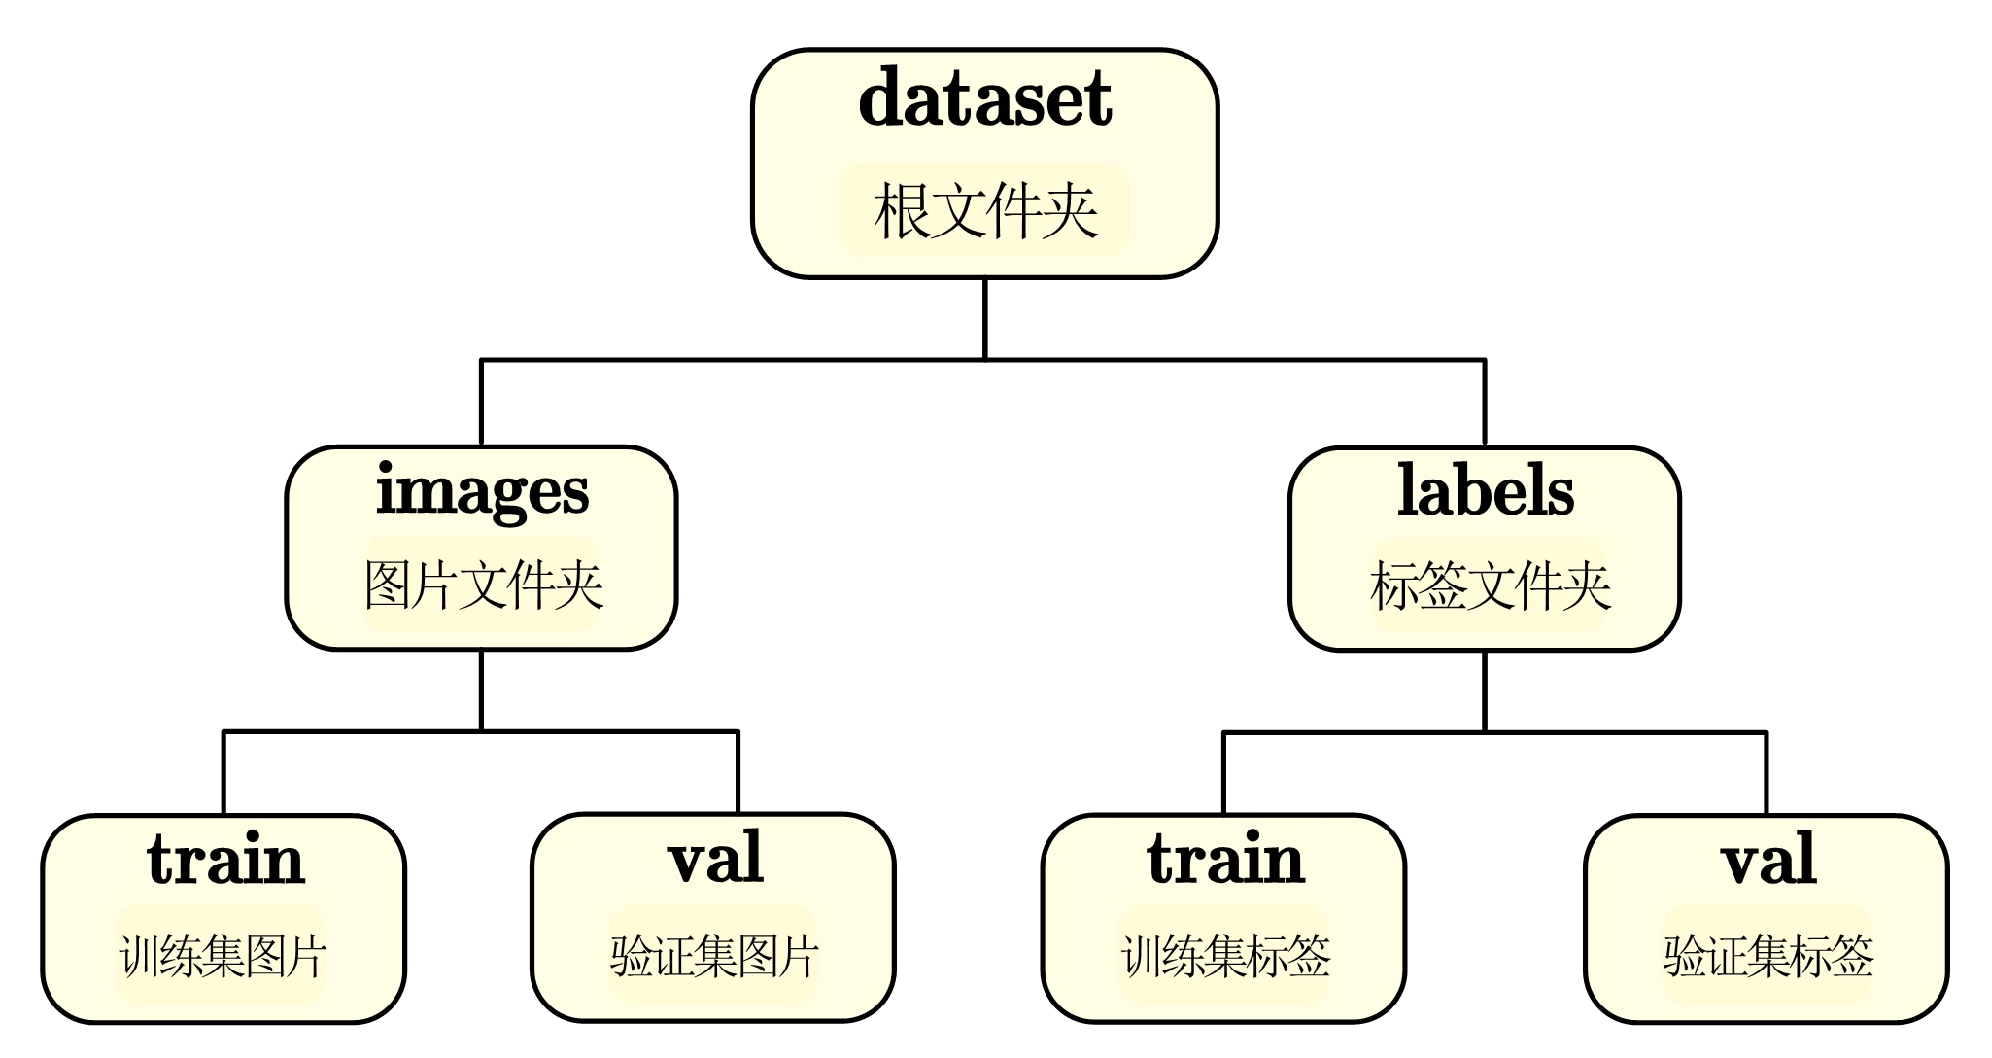
\includegraphics[width=0.48\textwidth]{figures/数据集结构图}
        \label{fig:dataset_structure}
    }
    \hfill
    \subfigure[labelImg软件标注界面]{
        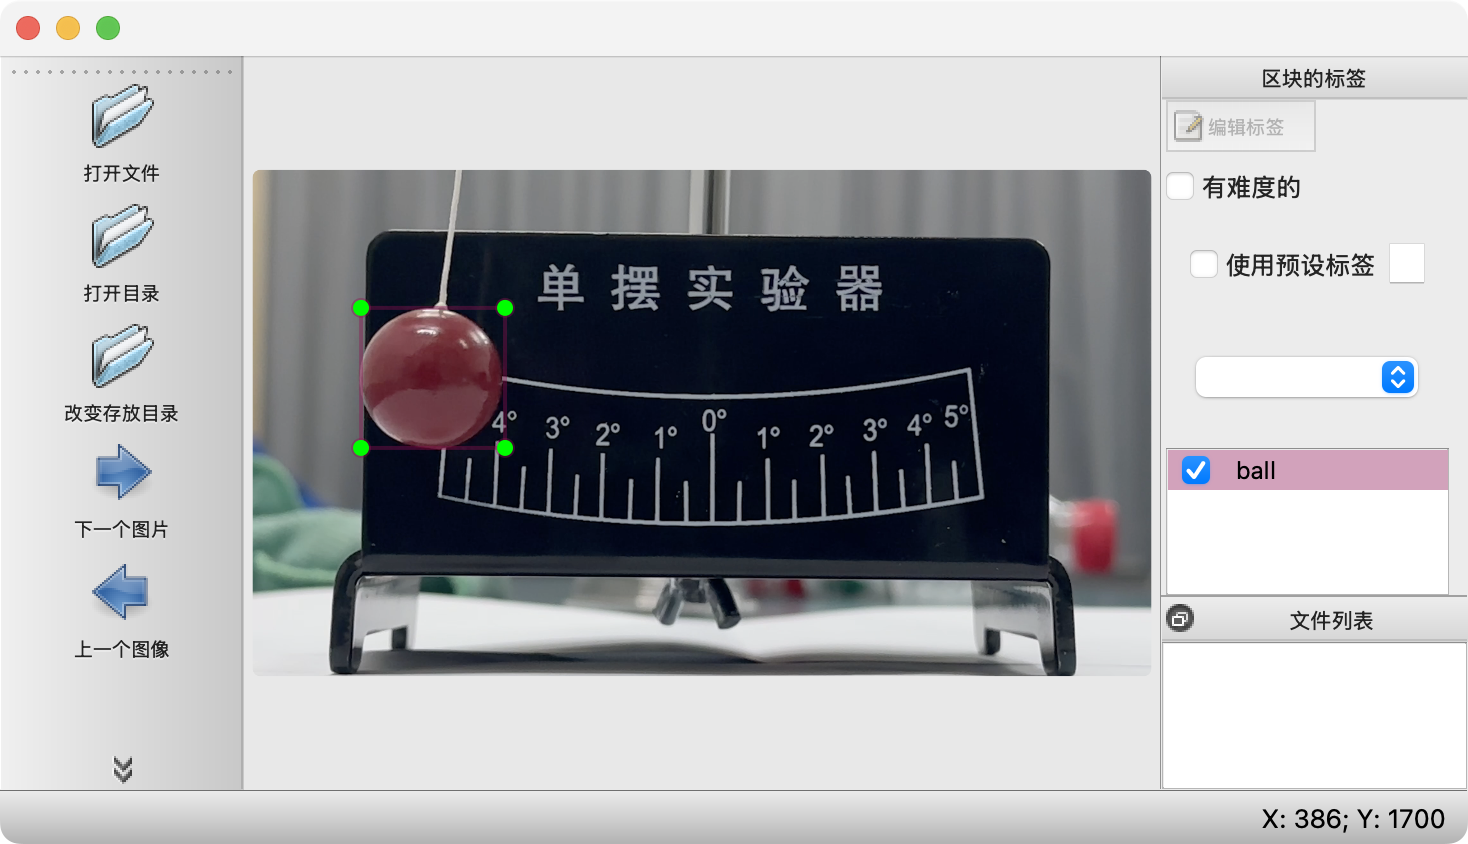
\includegraphics[width=0.48\textwidth]{figures/标注1.png}
        \label{fig:labelImg}
    }
    \caption{数据集标注与数据集目录结构}
    \label{fig:dataset}
\end{figure}

\subsubsection{模型的训练与评估}
本团队将epoch(训练轮数)设置为100,并开启多尺度训练增强训练的效果,最终到得到了最佳训练结果,保存为best.pt的权重文件。其 Loss 变化图如图\ref{fig:loss_change}所示。
可以看出,模型在前50次迭代中迅速拟合,后50次迭代后渐渐稳定,只有稍许震荡,说明训练效果较好。本团队另外拍摄了一段实验装置的视频,使用训练后的模型进行检测,\textbf{检测框全程稳定跟踪,置信度达到0.9以上},如图\ref{fig:video_test}所示,模型检测能力较好,可以用于后续的测量实验。
\begin{figure}[H]
    \centering
    \subfigure[Loss变化图]{ 
        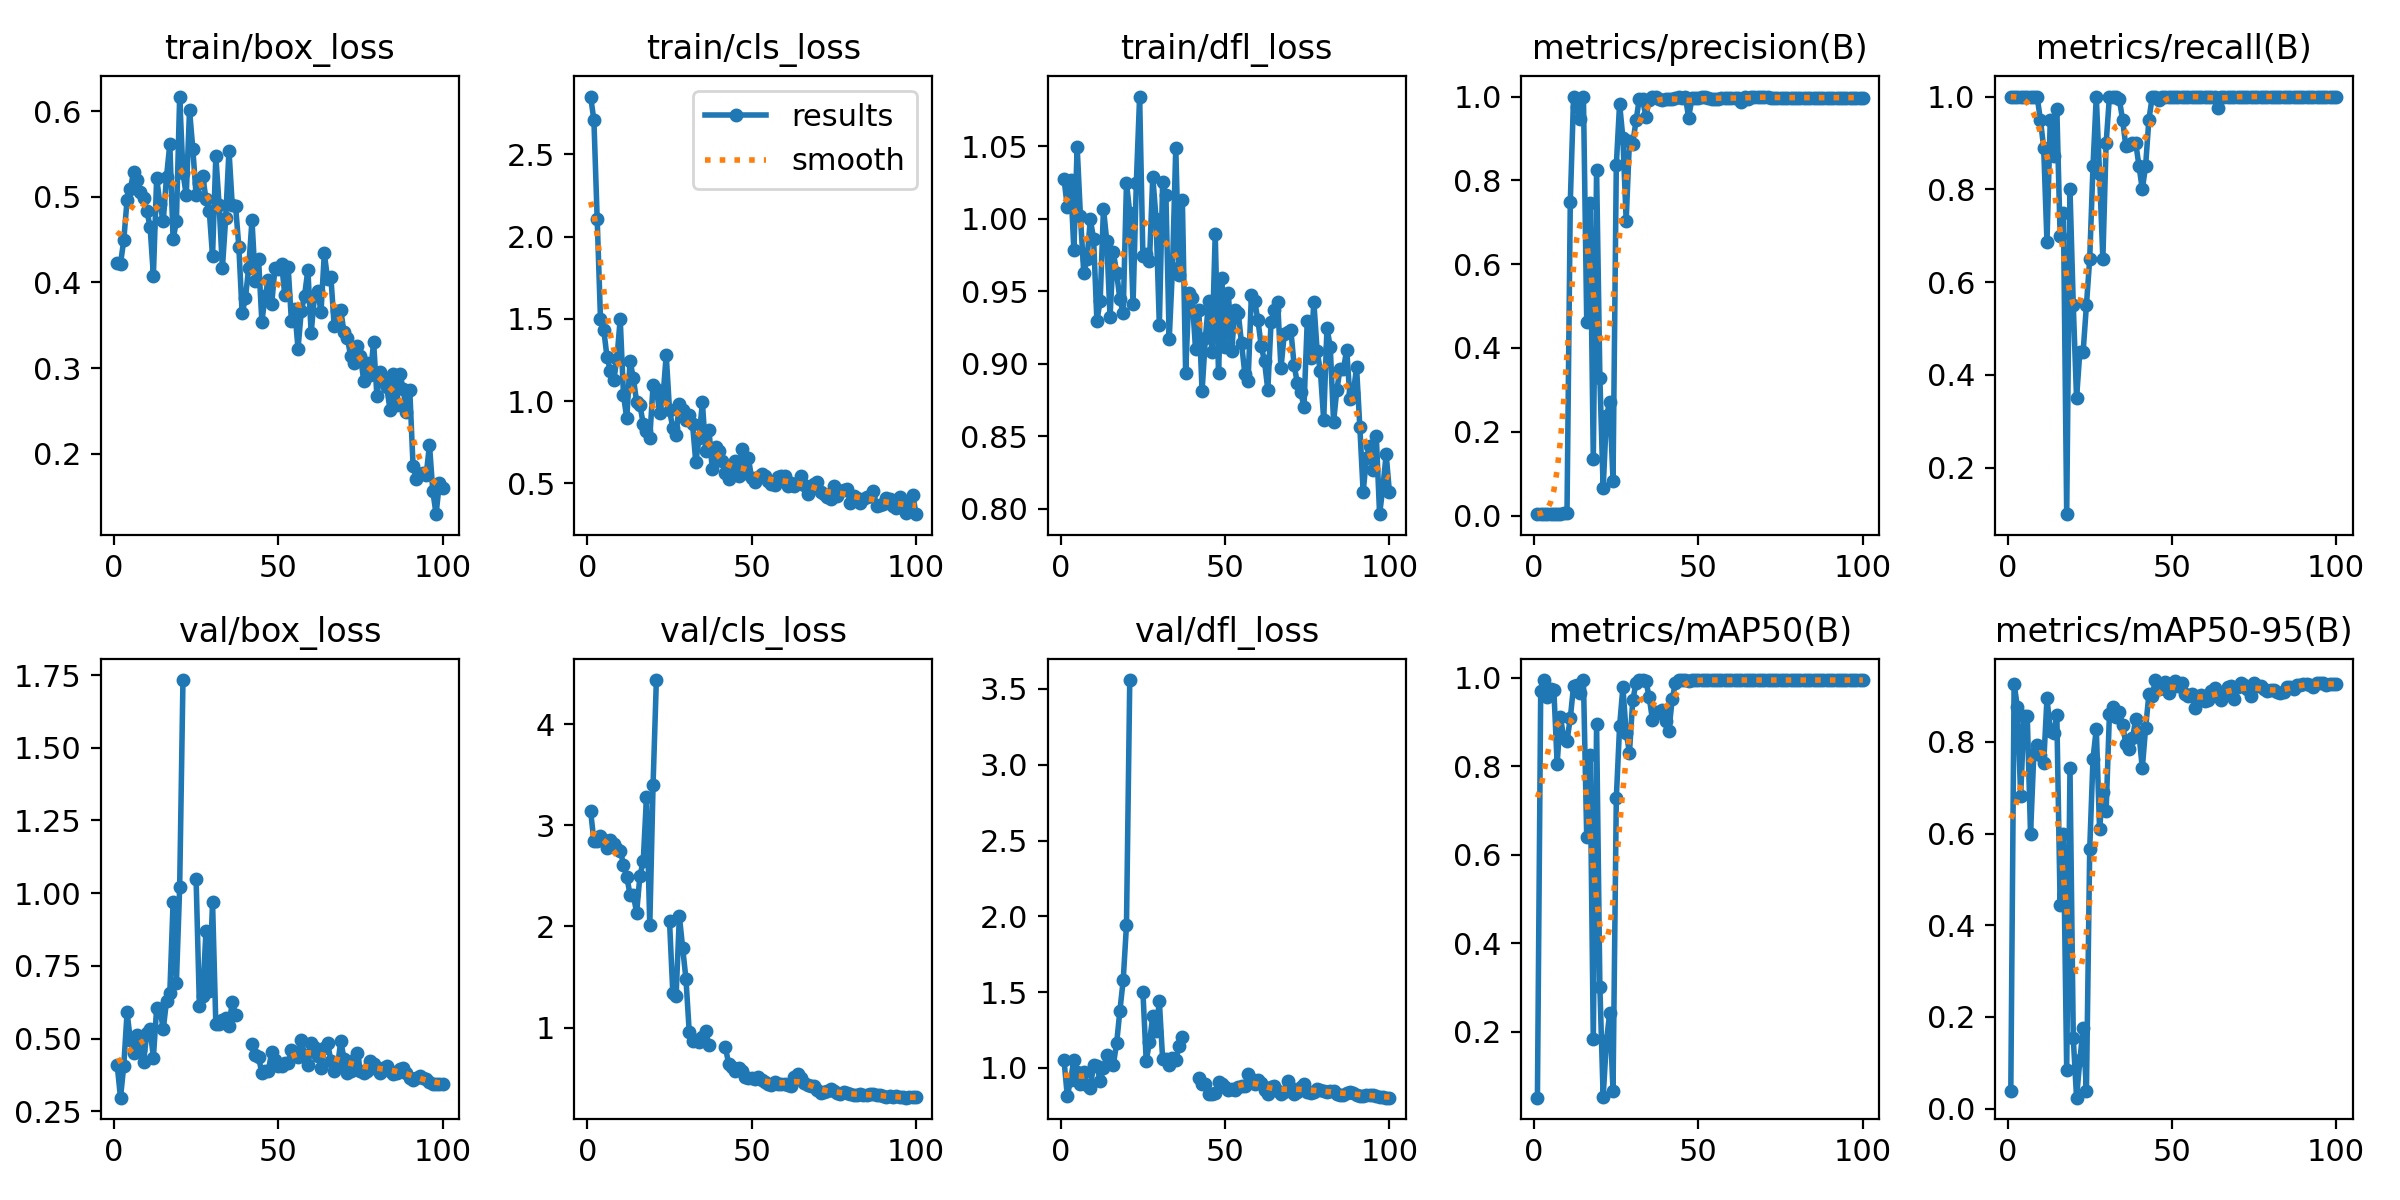
\includegraphics[width=0.55\textwidth]{figures/训练结果.png}
        \label{fig:loss_change} 
    }
    \subfigure[测试视频的检测结果]{
        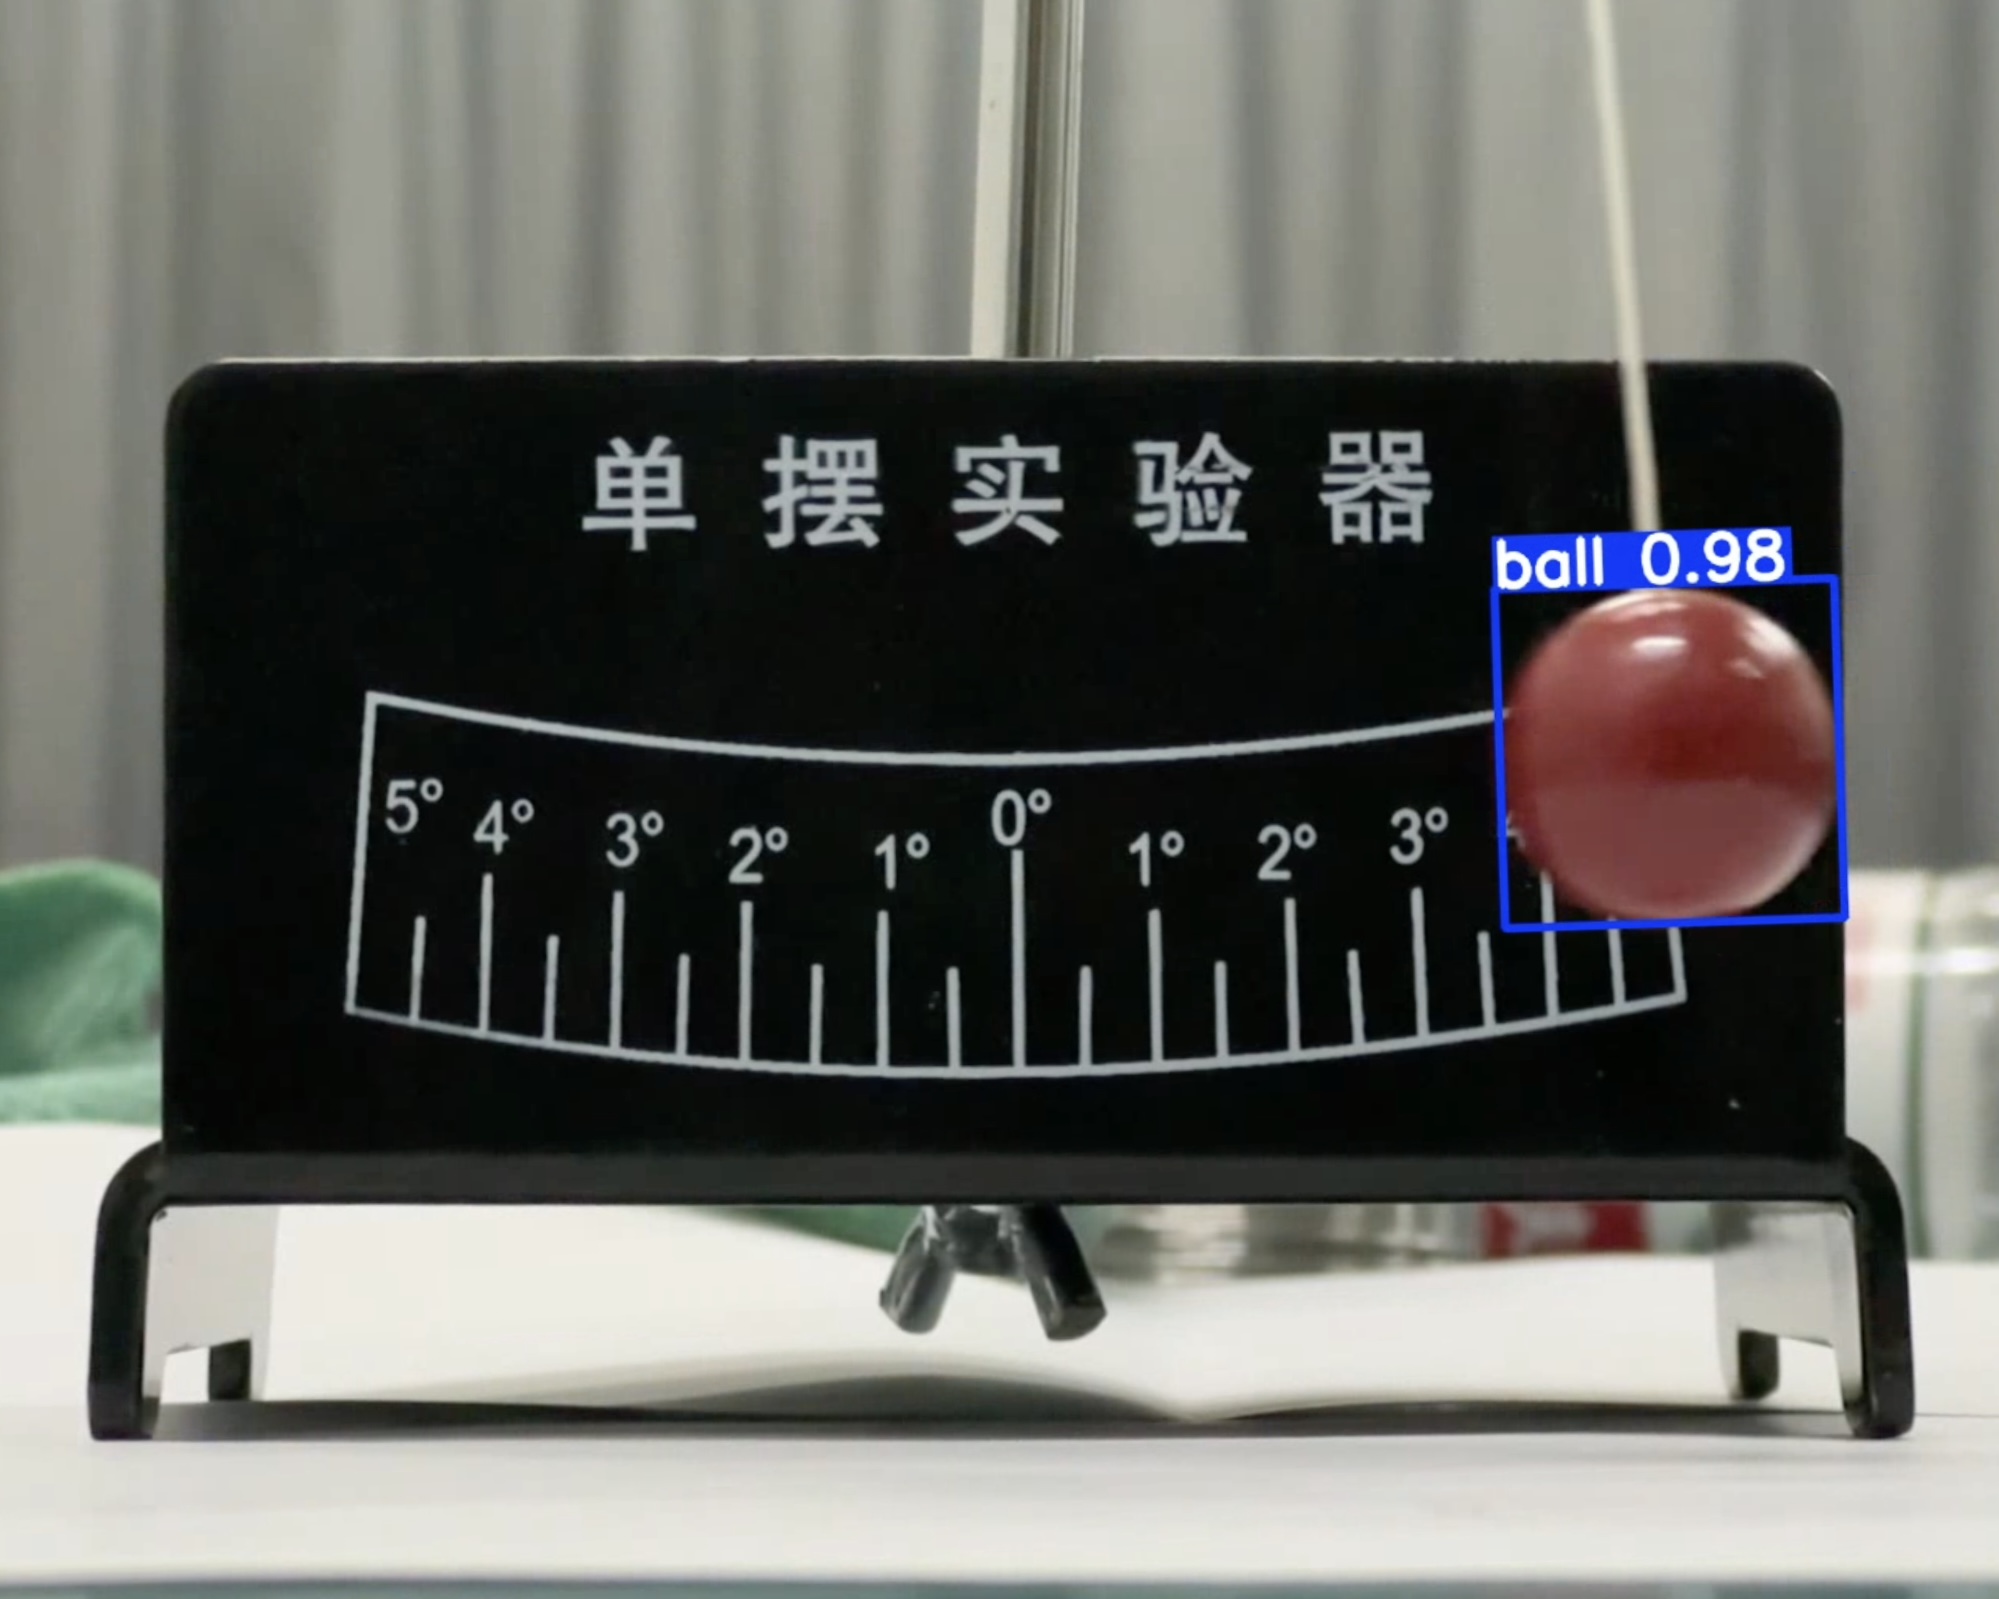
\includegraphics[width=0.35\textwidth]{figures/摆球识别效果2}
        \label{fig:video_test}
    }
    \caption{模型训练结果与识别效果}
    \label{fig:test_result}
\end{figure}

\subsubsection{软件设计}

在训练出能够精准识别摆球的AI模型后,本团队开发了一款集成相关功能的软件,便于其在实验中应用。本软件使用Python编写,依赖于多个第三方库,如PySide6(用于构建图形用户界面)、OpenCV(用于视频和图像处理)、ultralytics(包含YOLO模型,用于目标检测)、numpy、pandas、scipy(用于数值计算)以及matplotlib(用于绘图和数据可视化)。软件采用\textbf{模块化设计,各模块功能分离,便于维护和扩展},其结构图如图\ref{fig:software_structure}所示,包含三个主要模块:\texttt{gui.py}、\texttt{tracker.py} 和 \texttt{analyzer.py},源代码见附录\ref{app:software_code}。
下面将详细介绍每个模块的功能。

\begin{figure}[H]
    \centering
    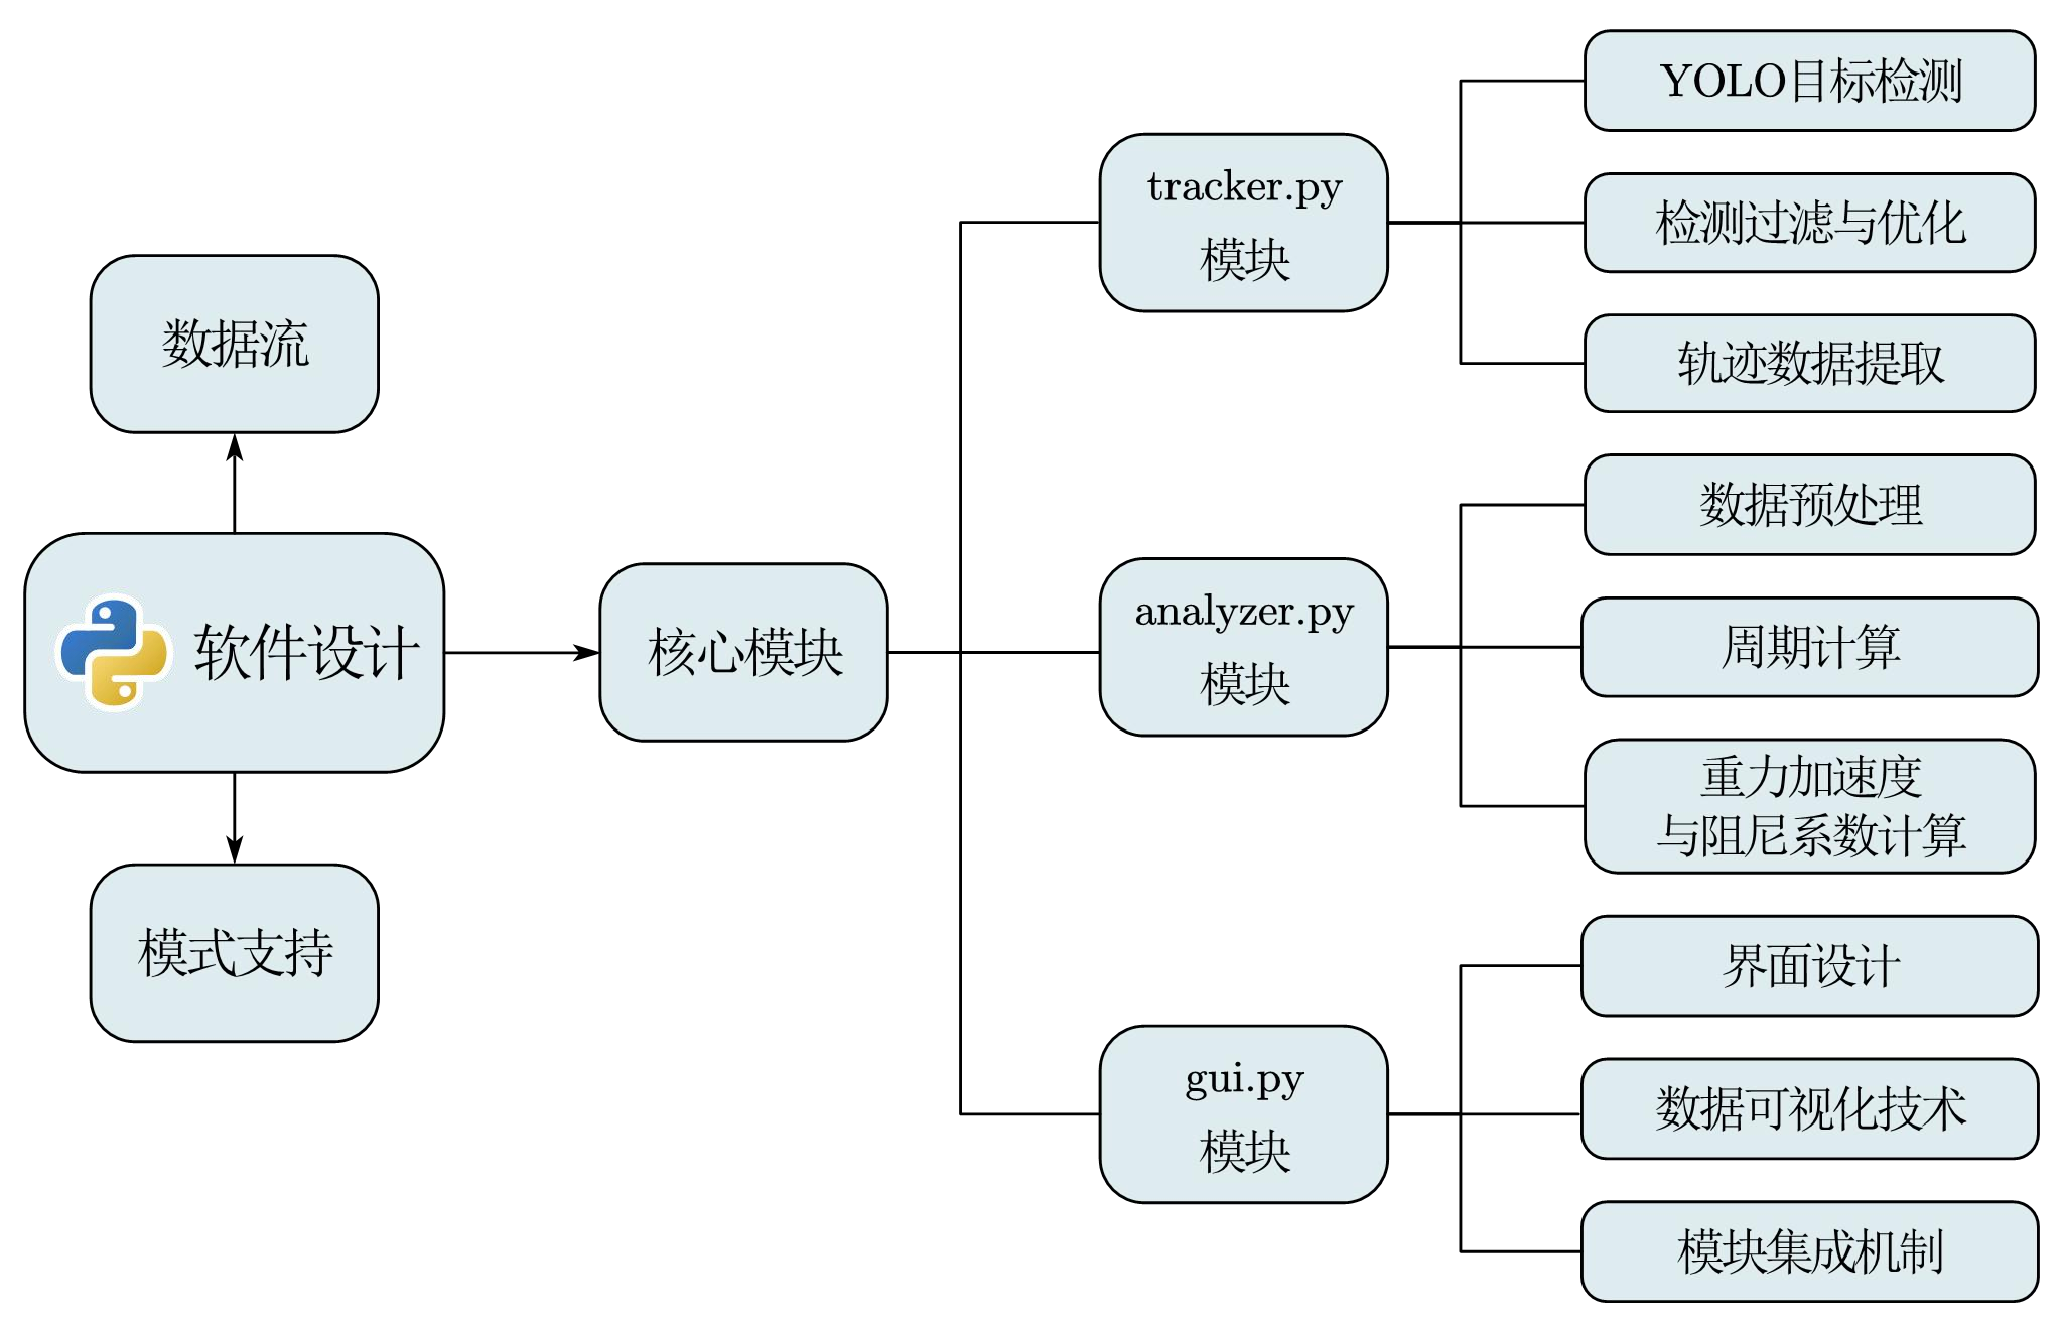
\includegraphics[width=0.7\textwidth]{figures/软件结构图.pdf}
    \caption{软件结构图}
    \label{fig:software_structure}
\end{figure}

\textbf{tracker.py模块},该模块负责目标检测和视频数据处理,实现小球的自动追踪与位置记录,完成\textbf{物理现象的观察}。其核心算法包括:
\begin{enumerate}
\item YOLO目标检测:系统运用YOLO深度学习模型实现单摆小球的快速识别。YOLO模型将图像分割为网格,每个网格预测边界框和类别概率,最终通过非极大值抑制(NMS)算法过滤重叠边界框,实现物体定位。相比传统计算机视觉方法,YOLO能够适应不同光照条件和背景干扰,提高小球定位精度。
    
\item 检测过滤与优化:系统实现了基于时间连续性的检测过滤机制,通过比较连续帧之间的边界框大小变化,筛除异常检测结果。该算法使用滑动窗口存储历史检测框大小,并通过中位数过滤实现对摆球运动轨迹的平滑跟踪,有效解决了传统视频处理中因光照变化、运动模糊等因素导致的识别不稳定问题。
    
\item 轨迹数据提取:系统从YOLO检测结果中提取小球中心坐标,并将其与实验时间戳关联,生成时间-位置数据序列。这种方法实现了小球运动过程的高精度记录,相较于传统的手动计时和目测方法,大幅提高了数据采集的精度和效率。

\end{enumerate}
\begin{figure}[H]
    \centering
    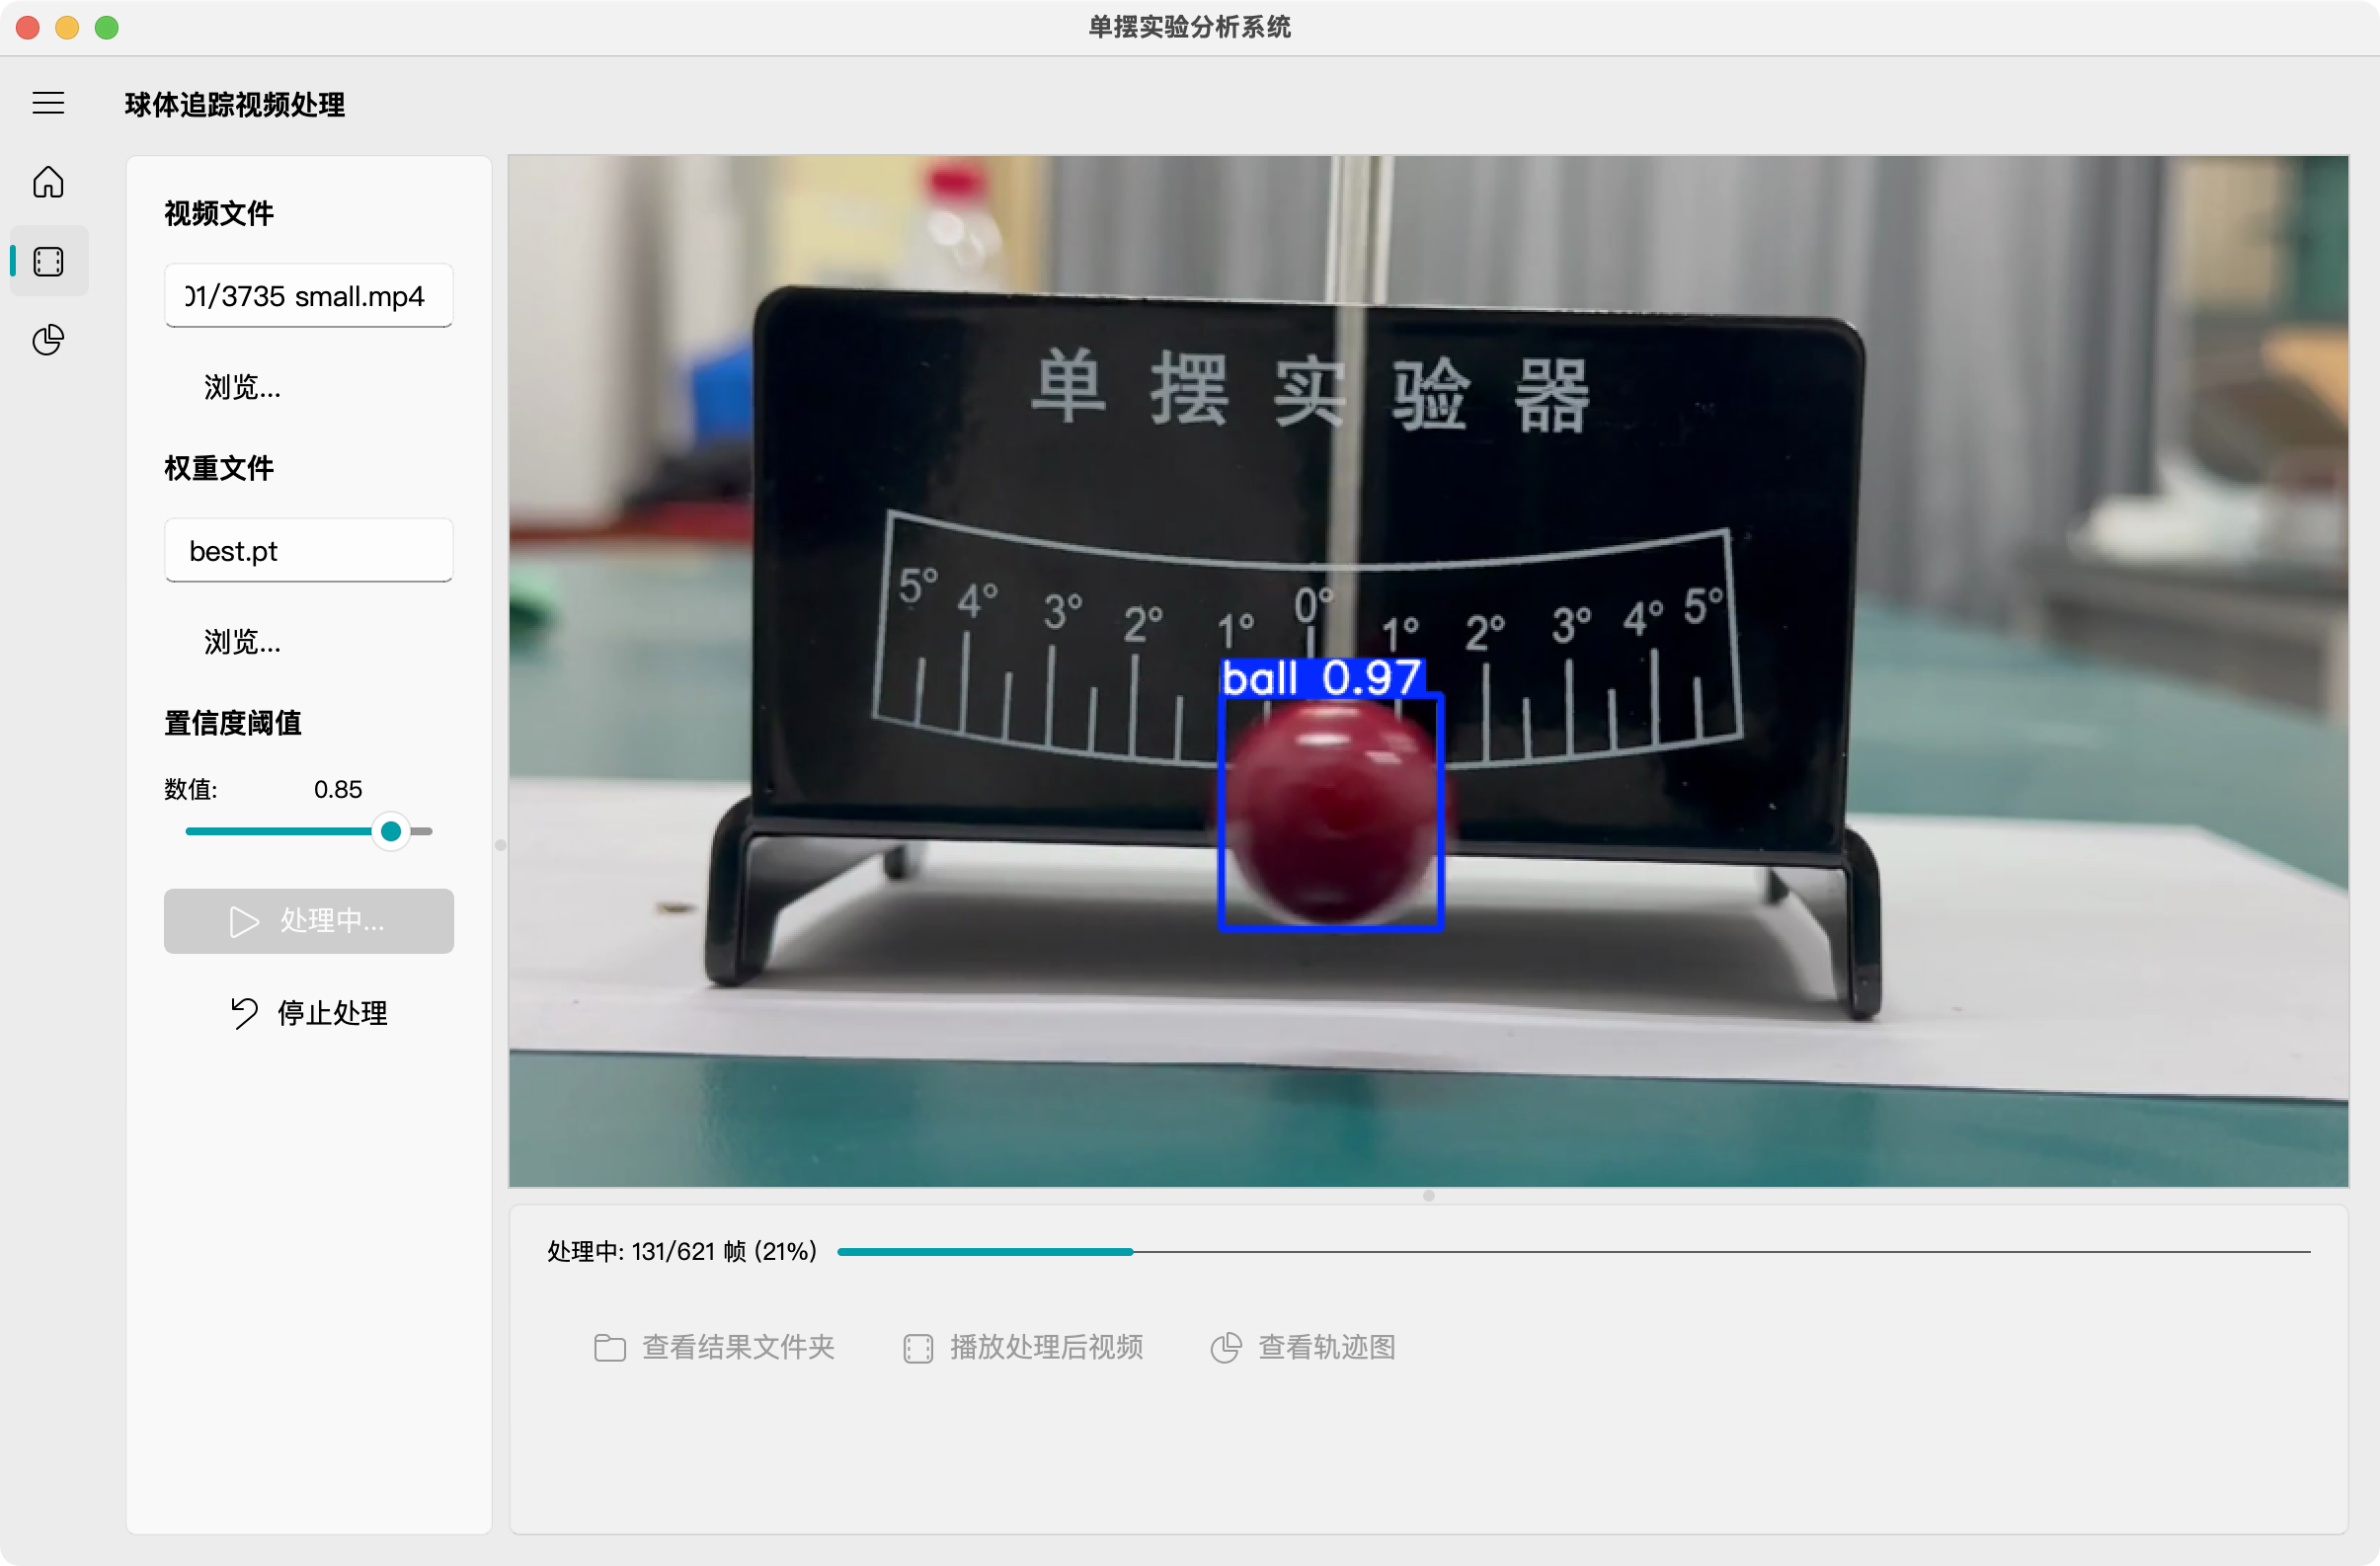
\includegraphics[width=0.5\textwidth]{figures/视频处理界面.png}
    \caption{视频处理界面}
    \label{fig:video_processing}
\end{figure}

\textbf{analyzer.py模块},该模块负责对轨迹数据进行物理分析,实现周期测量、重力加速度和阻尼系数等\textbf{物理参数的计算}。核心算法包括:
\begin{enumerate}
\item 数据预处理:系统采用Savitzky-Golay滤波器进行数据平滑,该滤波器通过局部多项式最小二乘拟合实现信号降噪。其核心思想是在时域上对数据点应用移动窗口,在每个窗口内使用多项式拟合局部数据,进而获得滤波点。与简单移动平均不同,该方法能够较好地保留信号的高频特征(如峰值和快速变化),同时有效抑制噪声,特别适合处理周期性运动数据。
    
\item 周期计算方法:系统提供三种互补的周期分析方法,实现高精度周期测量:
    \begin{enumerate}[label=\alph*.]
        \item 快速傅里叶变换(Fast Fourier Transform,FFT)分析法\textsuperscript{\cite{9787115284846001}}:该方法首先将时域信号转换到频域,通过分析频谱中的能量分布,识别出主频率。FFT分析特别适用于包含多频率成分的信号,但对于时间序列有限的情况,可能存在频率分辨率的限制。为提高精度,系统采用了汉宁窗(Hanning window)预处理信号并进行零填充(zero-padding),增强频谱分析的频率分辨率;
        
        \item 峰值检测法:该方法直接在时域上工作,通过识别位移-时间曲线中的局部极大值点(峰值),计算相邻峰值间的时间差作为周期估计。系统通过设置最小峰值距离和显著性阈值(prominence)参数,提高了峰值检测的准确性。该方法直观且计算效率高,但对噪声较为敏感;
        
        \item 曲线拟合法:该方法基于单摆的理论模型,通过最小二乘法将简谐运动方程 $x(t) = A\sin(\omega t + \phi) + C$ 拟合到实验数据。该方法利用整个数据集信息,对噪声具有较强的鲁棒性,且能同时提取振幅、频率和相位等多个参数,但计算复杂度较高,且依赖于初始参数估计。
    \end{enumerate}
    
  
\item 重力加速度计算:根据单摆理论,周期$T$与摆长$l$和重力加速度$g$的关系为$T = 2\pi\sqrt{l/g}$。系统基于此公式,结合周期测量结果,计算得到重力加速度$g = 4\pi^2l/T^2$。为提高大摆角条件下的计算精度,系统还实现了非线性周期修正,考虑摆角$\theta$的影响:$T = T_0(1 + \frac{1}{16}\theta^2 + \frac{11}{3072}\theta^4 + ...)$,其中$T_0$为小摆角条件下的理论周期。
    
\item 阻尼系数计算:系统采用对数衰减法计算阻尼系数。
    在单摆系统中,空气阻力产生的阻尼使振动振幅随时间呈指数衰减:$A(t) = A_0e^{-\frac{\beta}{m} t}$,其中$\beta$为阻尼系数,$m$为摆球质量。
    根据实验数据,系统首先提取振动峰值点,获得一系列时间-振幅数据对$(t_i, A_i)$,然后基于公式$\beta = \frac{m}{nT}\ln\frac{A_0}{A_n}$计算阻尼系数,
    其中$n$为周期数,$T$为平均周期,$A_0$为初始振幅,$A_n$为$n$个周期后的振幅。系统还计算了相关参数:固有频率$\omega_0 = 2\pi/T$、
    品质因数$Q = \omega_0/(\beta/m)$及衰减时间常数$\tau = m/\beta$。为直观展示衰减规律,系统对振幅取对数后进行线性拟合,斜率即为阻尼系数与质量比值$\beta/m$的相反数,
    通过可视化对比理论与实测的衰减曲线,验证了阻尼模型的有效性。该方法能够有效表征空气阻力对单摆运动的影响,为阻尼振动研究提供定量分析手段。
\end{enumerate}

\begin{figure}[H]
    \centering
    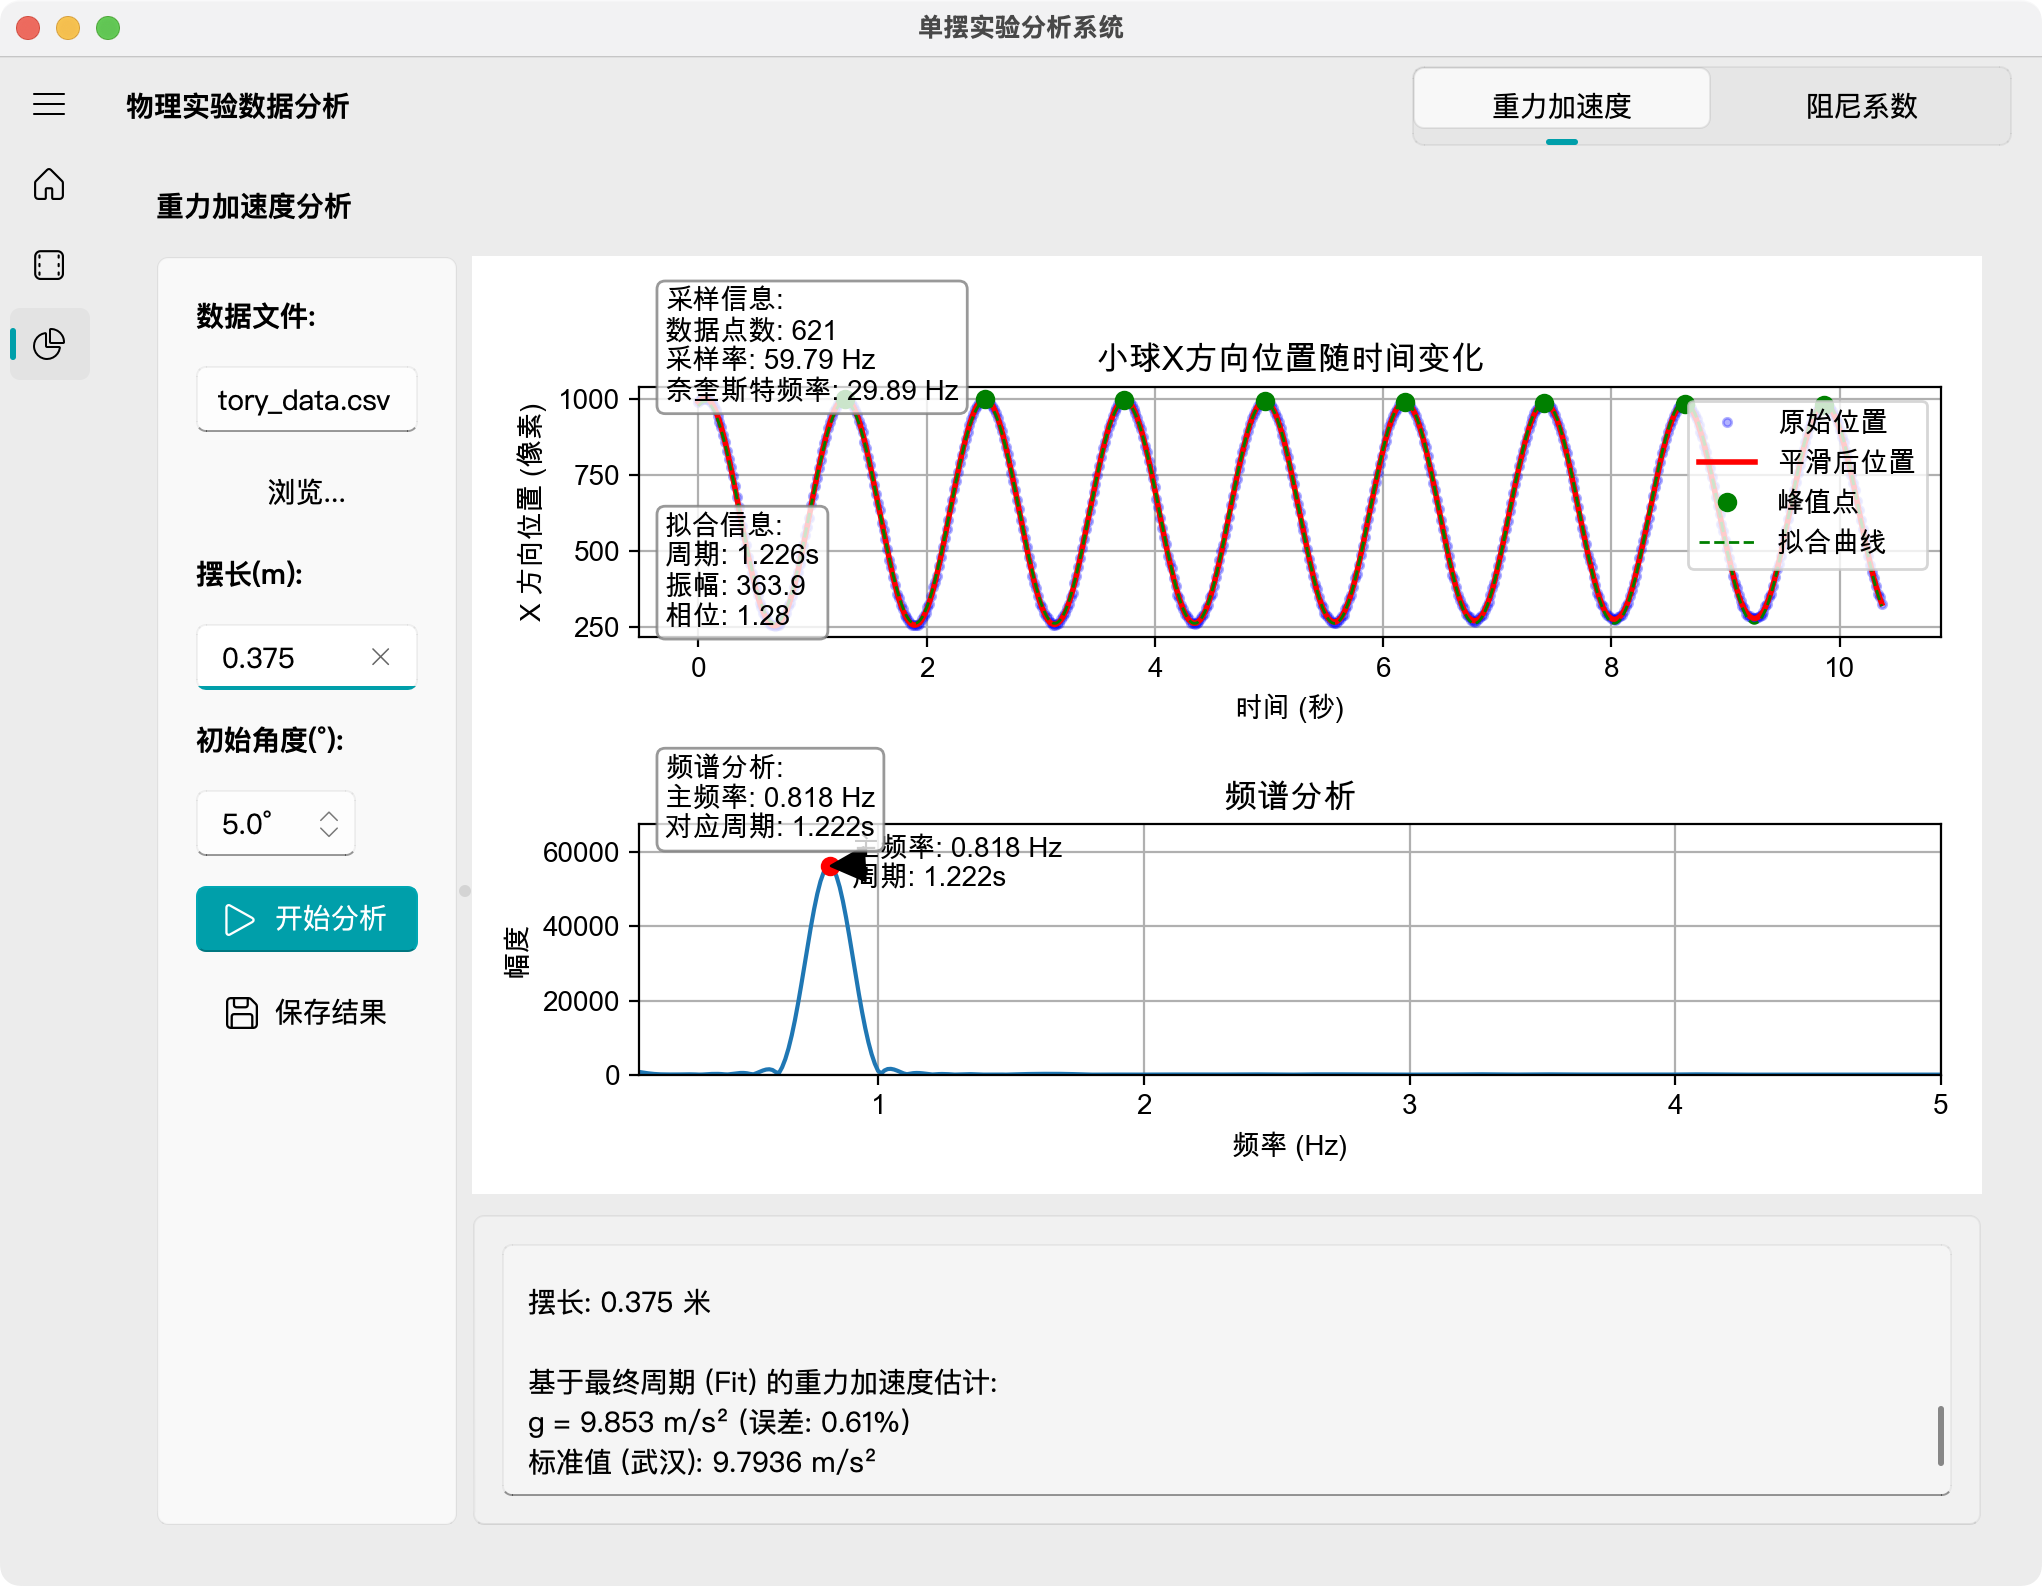
\includegraphics[width=0.5\textwidth]{figures/数据分析界面.png}
    \caption{数据分析界面}
    \label{fig:data_analysis}
\end{figure}

\textbf{gui.py模块},该模块实现了整体用户界面,设计了\textbf{直观的交互流程}和\textbf{数据可视化}功能:

\begin{enumerate}
    \item 界面设计:软件采用流体设计语言(Fluent Design),通过亚克力效果(高斯模糊与透明度混合)创建深度感和层次感,增强用户体验。界面组件如导航栏、卡片和按钮均采用圆角设计,配合动态阴影和悬停效果,提供现代化的视觉体验。      
    \item 数据可视化技术:系统整合matplotlib绘图库,设计了多种可视化图表:
    \begin{enumerate}[label=\alph*.]
        \item 轨迹图:展示小球在二维平面内的运动轨迹,直观反映运动范围和路径;
        \item 位置-时间图:展示位置随时间变化的曲线,并叠加拟合曲线,便于观察振动特性;
        \item 频谱分析图:展示信号频谱,标记主频点,帮助理解振动的频率组成;
        \item 对数衰减图:展示振幅对数值随时间的变化,用于直观观察阻尼特性。
    \end{enumerate}
    
    \item 模块集成机制:系统通过Qt的信号槽机制实现模块间松耦合集成。视频处理完成后自动触发分析模块,分析结果实时更新到界面,形成完整的工作流。这种设计使用户能够在同一界面中完成从视频导入到结果查看的全部操作,大幅提升了实验效率。
\end{enumerate}


\begin{figure}[H]
    \centering
    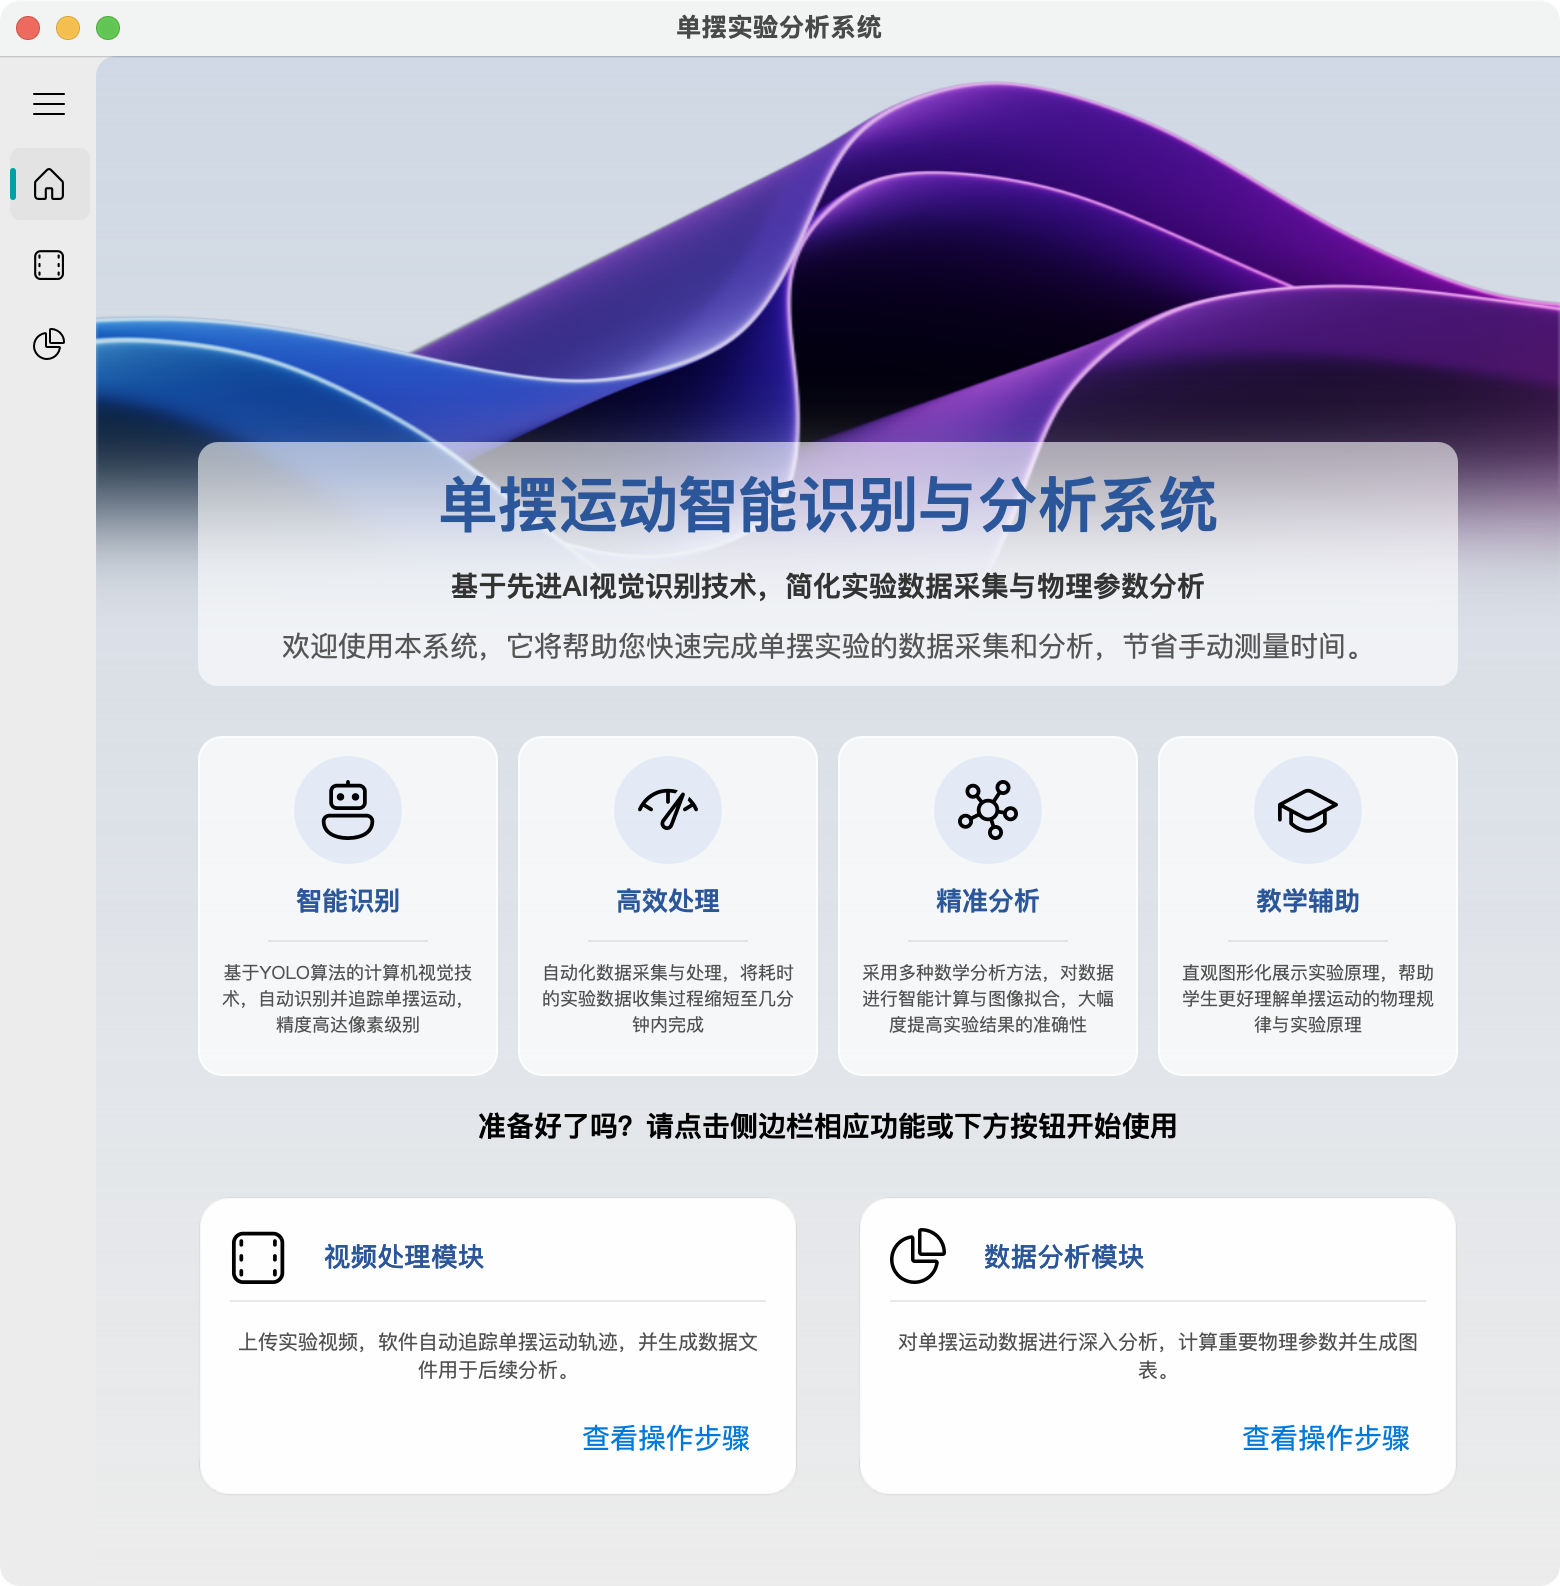
\includegraphics[width=0.5\textwidth]{figures/软件界面1.png}
    \caption{软件交互界面展示}
    \label{fig:software_interface}
\end{figure}


通过这种模块化设计,软件实现了从物理现象的观察到物理参数计算的完整流程,使用户能够直观地获取实验数据,进行周期和重力加速度的计算,并可视化实验结果,有效地将AI技术与物理实验教学相结合。

\subsection{系统误差分析}

在实验过程中,除了理论模型和算法带来的误差外,系统性误差也可能影响测量的准确性。这些误差来源多样,涵盖了图像采集和处理、数据处理算法、物理系统、环境因素以及基准值误差等方面。下面将详细分析各类误差的来源及其对实验结果的可能影响。

\subsubsection{图像采集和处理误差}  
在图像采集和处理阶段,主要的误差来源包括以下几点:
(1)YOLO目标检测的定位误差:即使在理想条件下,YOLO目标检测算法也存在一定的误差,这可能导致小球位置的测量不够精确;
(2)摄像机的帧率限制:由于摄像机的帧率有限,采样点可能不足以充分捕捉到小球运动的细节,从而影响周期的准确测量;
(3)摄像机的视角误差:如果摄像机未能完全垂直于单摆的运动平面,则会产生投影误差,进而影响位置的测量;
(4)镜头畸变:相机镜头的畸变可能在图像边缘产生系统性偏差,这些畸变可能导致边缘区域的位置测量不准确,进而影响整个实验的结果。

\subsubsection{数据处理算法误差}  
在数据处理过程中,主要的误差来源有以下几点:
(1)平滑处理带来的误差:使用Savitzky-Golay滤波器进行数据平滑时,虽然有效地减少了噪声,但也可能稍微改变信号的相位和幅度,从而影响周期的测量;
(2)FFT分析的频率分辨率问题:FFT分析的频率分辨率限制可能导致无法准确捕捉低频信号;
(3)峰值检测误差:峰值检测法在噪声较大的情况下可能出现误判,导致周期测量误差;
(4)曲线拟合误差:曲线拟合假设简谐运动模型,但实际运动受阻尼等因素影响,模型与实际情况的不完全契合可能导致周期测量误差。

\subsubsection{物理系统误差}  
物理系统中的误差主要来源于以下几个方面:
(1)大摆角误差:本实验的测量原理是基于小摆角近似,但实际实验中如果摆角较大,会导致测量结果存在误差,虽然程序中采用了大摆角修正,但该修正公式依然是近似的;
(2)摆长测量误差:摆长被定义为从支点到摆球质心的距离,但由于摆球并非理想质点,且绳子本身具有一定的弹性,这些因素可能导致摆长测量不准确,进而影响重力加速度的计算;
(3)空气阻力影响:实验模型假设了简谐运动,但实际上空气阻力会导致振幅逐渐减小,从而影响周期的测量,特别是在较长时间的实验中,空气阻力的影响不可忽视。


\subsubsection{环境因素}  
环境因素是另一重要的误差来源,具体包括以下几点:
(1)温度变化对摆长的影响:温度变化可能导致绳子长度的微小变化,进而影响周期的测量精度;
(2)空气密度变化:空气密度的变化会影响空气阻力的大小,进而影响实验结果;
(3)支点摩擦:理想情况下假设支点无摩擦力,但实际上支点摩擦力矩的存在会影响小球的运动,进而影响测量结果;
(4)外部振动:实验环境中的外部震动可能影响测量的精度,尤其在高精度测量中,这一因素的影响需要特别注意。

\subsubsection{基准值误差}  
基准值误差主要体现在重力加速度的基准值选择上。代码中使用的是武汉地区的标准重力加速度(9.7936 m/s²),但实际实验地点的重力加速度可能存在差异。具体来说,实验地点的海拔高度和纬度等因素会影响当地的重力加速度值,这可能导致实验结果的误差。 